%#! platex thesis.tex

%======================================================================
\chapter{LSTMを用いた手書き医療用語認識とSRP手法及びRatio手法によるデータ拡張}
\label{cha:propose}
本章では,先行研究\cite{takahashi}のBidirectionalLSTMを用いたオンライン手書き医療用語認識を説明する.また,オンライン文字認識用のデータ拡張手法として先行研究のSRP手法を説明し,データ拡張の新手法としてRatio手法を提案する.
%----------------------------------------------------------------------
\section{システムの概要}
\label{sec:concept}
\textbf{図~\ref{sys_concept}} にシステムの概要を示す.提案システムでは,タブレットから収集した手書き医療用語の座標データに対して前処理を行う.その後学習プロセスでは前処理後のデータに拡張手法を適用し,機械学習における学習データとする.推定プロセスでは,学習を行ったモデルに前処理後のデータを入力し,用語を推定する.ニューラルネットワーク構造とデータ前処理,特徴量抽出に関しては\ref{ssec:drawing}項の文献\cite{takahashi}を参考にした.以下,各手順について述べる.

\begin{figure}[tb]
 \begin{center}
  \resizebox{\columnwidth}{!}{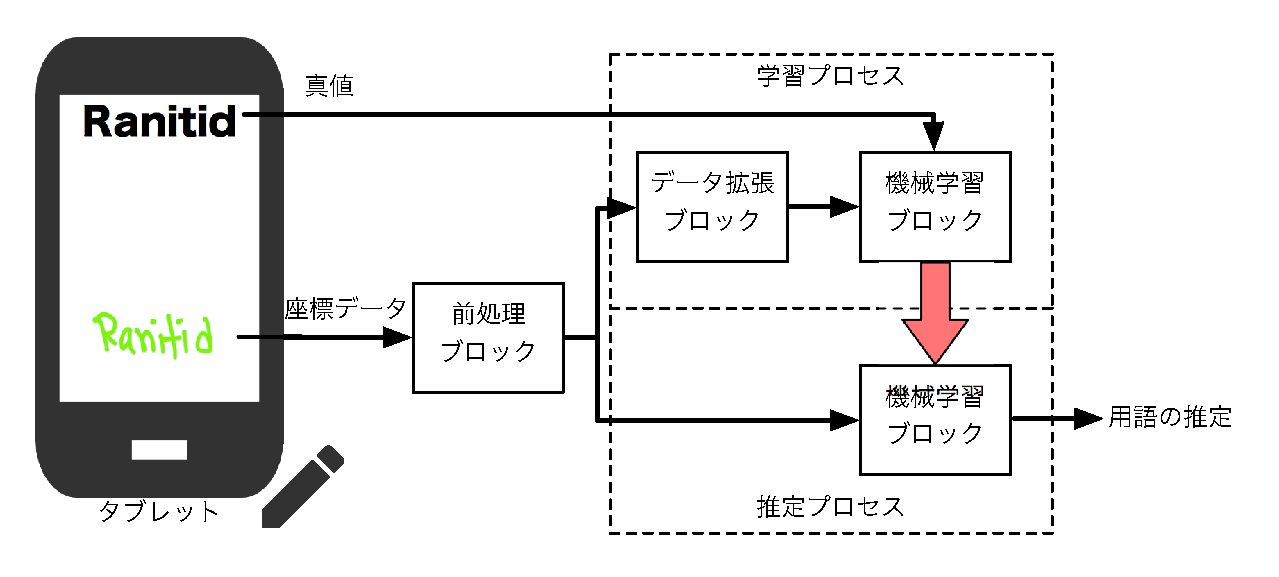
\includegraphics{img/system_structure.eps}}
  \caption{提案システムの概要}
  \label{sys_concept}
\end{center}
\end{figure}

\section{前処理ブロック}
\label{preprocess}
\textbf{図~\ref{preprocess}} に前処理ブロックの概要を示す.前処理ブロックでは,点の除去,正規化,特徴量抽出を行う.直線上の点や近接する点といった,取り除いても文字として成り立つような点の除去を行い,その後正規化を行う.特徴量抽出では点データを直線データへ変換する.以下,前処理ブロックにおける各処理を示す.

\begin{figure}[tb]
 \begin{center}
  \resizebox{\columnwidth}{!}{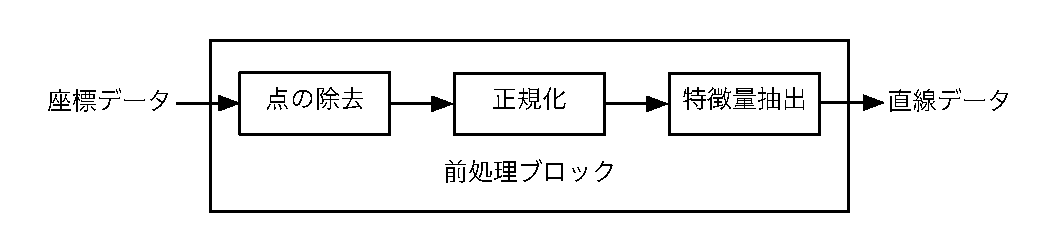
\includegraphics{img/preprocess.eps}}
  \caption{前処理ブロックの概要}
  \label{preprocess}
\end{center}
\end{figure}

\subsection{余分な点の除去}
\label{remove_points}
\textbf{図~\ref{extra}(a)}にオリジナルの単語データの例と, \textbf{図~\ref{extra}(b)} に余分な点が除去された後の単語データの例を示す.
収集する医療用語手書きデータは,\textbf{図~\ref{original}}で示したように$(x, y)$座標の時系列データとして存在している.本論文では文献\cite{zhang18:drawing}に従って,これに各点の筆順情報$s$を合わせた$(x, y, s)$を収集する.1つの単語を式~\ref{dataSt}のように収集する.
\begin{equation}
 [[x_1, y_1, s_1], [x_2, y_2, s_2],..., [x_n, y_n, s_n]]
 \label{dataSt}
\end{equation}
$x_i$と$y_i$は点の座標,$s_i$はその点が何画目のストローク上にあるかを示したものである.

手書きデータは書くスピードの違いなどが原因で,同じ単語でもデータ提供者によって点の数が大きく異なってしまい,うまく認識ができない可能性がある.本論文では先行研究に従い,取り除いても文字として成り立つような点の除去を行うことでデータ提供者ごとの点の数の差を小さくする.

\begin{figure}[tb]
 \centering
  \begin{tabular}{c}
   \begin{minipage}[b]{0.5\hsize}
    \centering
    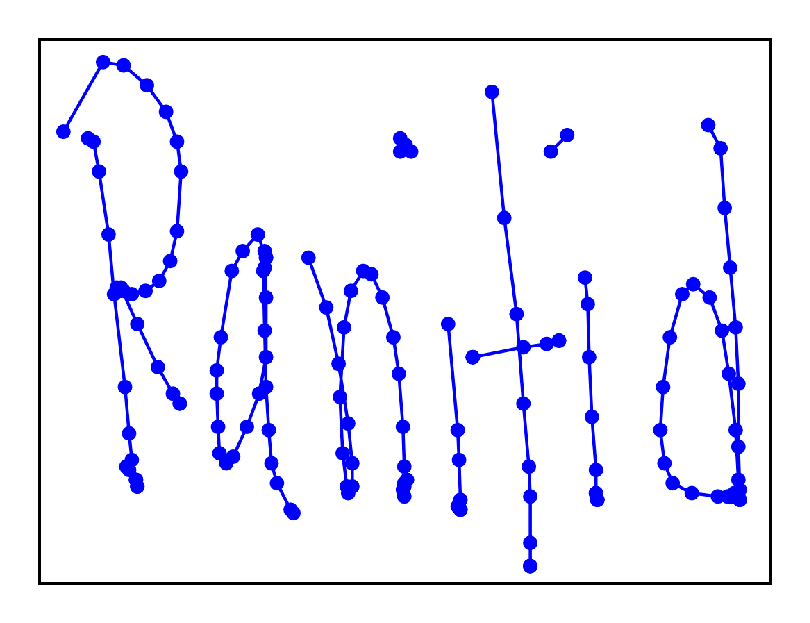
\includegraphics[keepaspectratio,scale=0.5]{img/ranitid.eps}\\
    (a)オリジナルデータ
   \end{minipage}\\
    % \hfill
   \begin{minipage}[b]{0.5\hsize}
    \centering
    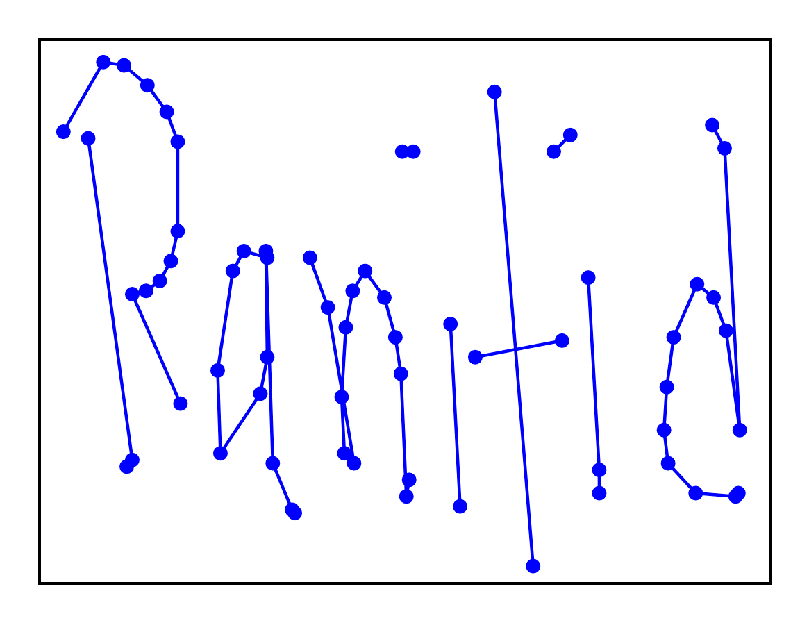
\includegraphics[keepaspectratio,scale=0.5]{img/ranitidClose.eps}\\
    (b)点の除去後
   \end{minipage}
  \end{tabular}
 \caption{データ前処理:余分な点の除去}
 \label{extra}
\end{figure}

\subsection{正規化}
\label{normal}
入力データをさらに簡潔にするため,点の除去を施したデータの正規化を行う.はじめに$x$座標についての正規化の手順を説明する.全てのデータの中から最大値$x_{max}$と最小値$x_{min}$を取り出し,式~\ref{eq:normalize}を用いてある点の$x$座標$X$を$X_{nor}$に正規化する.

\begin{equation}
  X_{nor} = \frac{X - x_{min}}{x_{max}-x_{min}}
  \label{eq:normalize}
\end{equation}
$y$座標に対しても同様の計算を行い,結果的に$(x, y)$をそれぞれ$0$以上$1$以下のデータとする.

\subsection{特徴量抽出}
\label{extract}
機械学習への入力のため,特徴量を抽出する.正規化した点データ2点間を繋ぎ,直線データを作成する.直線データに変換することで,点の座標だけでなく直線の長さ,角度などより多くの特徴量を抽出することができる.線データ$L_i$は,点$i$と点$i+1$から式~\ref{eq:line}のように構成され,本論文ではこのデータを学習における入力データとする.

\begin{equation}
  L_i = [x_i, y_i, \Delta{x_i}, \Delta{y_i}, I(s_i=s_{i+1}), I(s_i \neq s_{i+1})]
  \label{eq:line}
\end{equation}
ここで,$\Delta{x_i}=x_{i+1}-x_i$,$\Delta{y_i}=y_{i+1}-y_i$であり,$I()$は括弧内の条件が真であるときに$1$でありそれ以外では$0$である.$L_i$において$x_i$と$y_i$は直線の始点を表し,$\Delta{x_i}$と$\Delta{y_i}$は線の始点から終点までの$x$軸方向,$y$軸方向の距離を表す.また$I(s_i=s_{i+1})=1$は,直線の始点と終点が同一ストローク上にあることを示し,$I(s_i \neq s_{i+1})=1$はその直線で次のストロークに移ったことを示す.

%========================================================================
\section{データ拡張ブロック}
\label{augment}
ここでは様々な手書き文字に対応するためのデータ拡張について説明する.本研究では多様な提供者から大量のデータを得る必要があるが,十分なデータ量を確保するためには非常に多くの労力と時間を要する.そのため複数のデータ拡張手法を適用することで機械学習の際の手書き文字データの多様性を高める.はじめに先行研究のSRP手法を説明する.その後,文字の縦横比を変更する変更するRatio手法を提案する.

\subsection{SRP手法}
ここでは,先行研究\cite{takahashi}のデータ拡張手法であるStroke Rotation and Parallel-shift(SRP)手法について説明する.
SRP手法とは,ストロークの回転と平行移動によってデータ量を水増しする手法である.
\subsubsection{ストロークの回転}
ストロークの始点と終点の座標から中点を求め,その点を中心にストローク上の点をそれぞれ回転させることでストローク全体を回転させる.この処理を1つのデータに対して複数回施すことで,データ拡張を行う.

\textbf{図~\ref{rotate}(a)}にストロークの回転の原理を示す.ストロークの始点を$(x_f, y_f)$,終点を$(x_l, y_l)$とする.始点と終点の中点を$(a, b)$とすると,式~\ref{eq:center}より$(a, b)$の値が求められる.

\begin{equation}
  (a, b) = (\frac{x_f+x_l}{2}, \frac{y_f+y_l}{2})
  \label{eq:center}
\end{equation}
ストローク上の任意の点の座標を$(x, y)$としたとき,その点を,点$(a, b)$を中心に角$\theta$だけ移動させた後の座標$(X, Y)$は 式~\ref{eq:rotate}で表される.
\begin{equation}
  \left(
    \begin{array}{r}
        X-a \\
        Y-b
    \end{array}
    \right)
 = \left(
  \begin{array}{rr}
      cos\theta & -sin\theta \\
      sin\theta & cos\theta
  \end{array}
  \right)
  \left(
    \begin{array}{r}
        x-a \\
        y-b
    \end{array}
    \right)
  \label{eq:rotate}
\end{equation}
この式をストローク上のすべての点に用いることで,ストローク自体を角$\theta$回転させる.\textbf{図~\ref{rotate}(b)}にストローク回転前の単語データの例,\textbf{図~\ref{rotate}(c)}にストローク回転後の単語データの例を示す.この処理を,ストロークごとに角度を変えながら行うことで元のデータとは異なる形の文字・単語を生成する.それを1つの単語データに対して$N$回行い,データ量を$N$倍に拡張する.

\begin{figure}[tb]
 \centering
  \begin{tabular}{c}
   \begin{minipage}[b]{0.7\hsize}
    \centering
    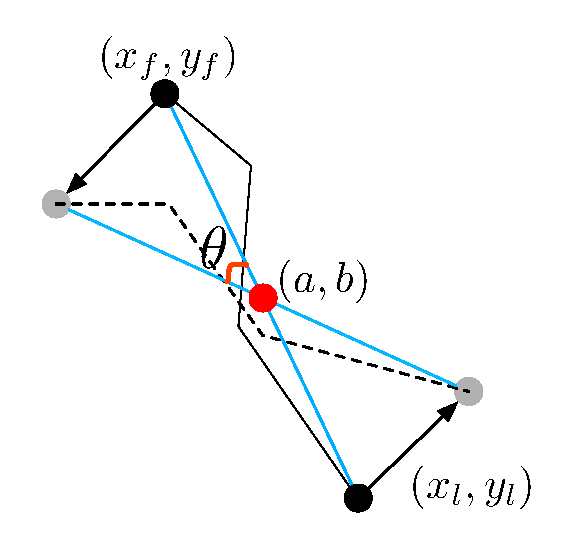
\includegraphics[keepaspectratio,scale=0.7]{img/rotate.eps}\\
    (a)回転の原理
   \end{minipage}\\
    \hfill
   \begin{minipage}[b]{0.5\hsize}
    \centering
    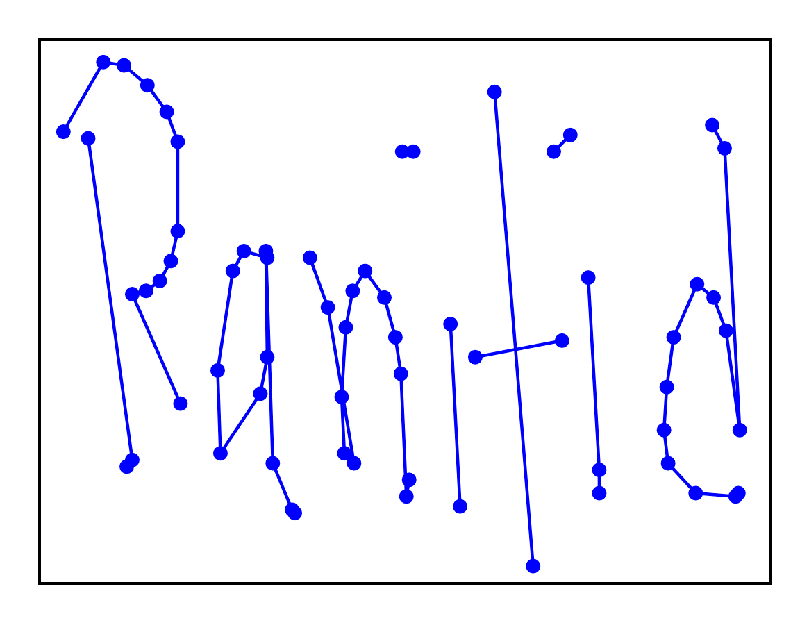
\includegraphics[keepaspectratio,scale=0.5]{img/ranitidCloseBlue.eps}\\
    (b)データ前処理後
   \end{minipage}
   \begin{minipage}[b]{0.5\hsize}
    \centering
    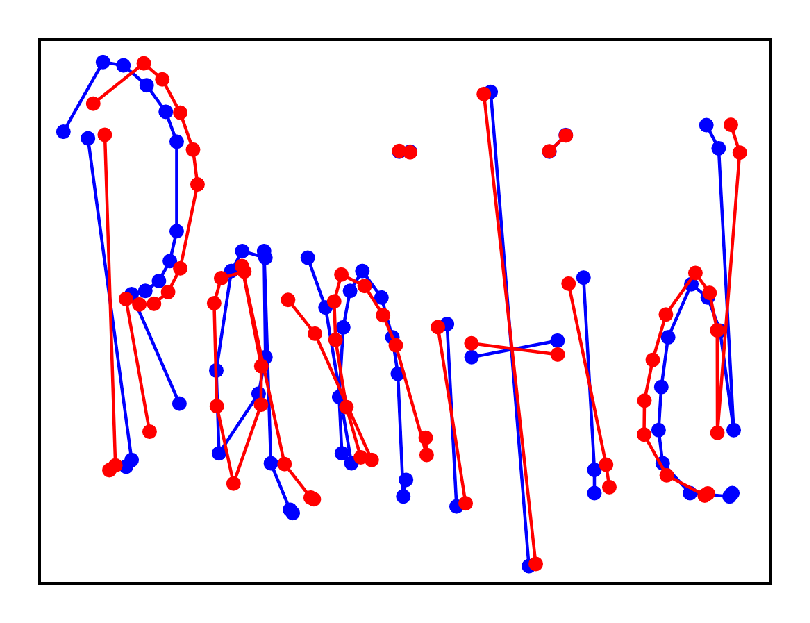
\includegraphics[keepaspectratio,scale=0.5]{img/ranitidRotateRedBlue.eps}\\
    (c)回転前(青)と回転後(赤)
   \end{minipage}
  \end{tabular}
 \caption{ストロークの回転}
 \label{rotate}
\end{figure}

\subsubsection{ストロークの平行移動}
ストローク上の点の座標それぞれに一定の値を加え,ストローク全体を平行移動させることでデータ拡張を行う.\textbf{図~\ref{parallel}(a)}にストロークの平行移動の原理を示す.ストローク上の任意の点の座標を$(x, y)$としたとき,その点を$x$方向に$dx$,$y$方向に$dy$だけ平行移動させた後の座標$(X, Y)$は 式~\ref{eq:parallel}で表される.

\begin{equation}
  (X, Y) = (x+dx, y+dy)
  \label{eq:parallel}
\end{equation}
この式をストローク上のすべての点に用いることで,ストローク自体を$x$方向に$dx$,$y$方向に$dy$平行移動させる.\textbf{図~\ref{parallel}(b)}にストローク平行移動前の単語データの例,\textbf{図~\ref{parallel}(c)}にストローク平行移動後の単語データの例を示す.この処理を,ストロークごとに$dx$と$dy$の値を変えながら行うことで元のデータとは異なる形の文字・単語を生成する.それを1つの単語データに対して$N$回行い,データ量を$N$倍に拡張する.

\begin{figure}[tb]
 \centering
  \begin{tabular}{c}
   \begin{minipage}[b]{0.7\hsize}
    \centering
    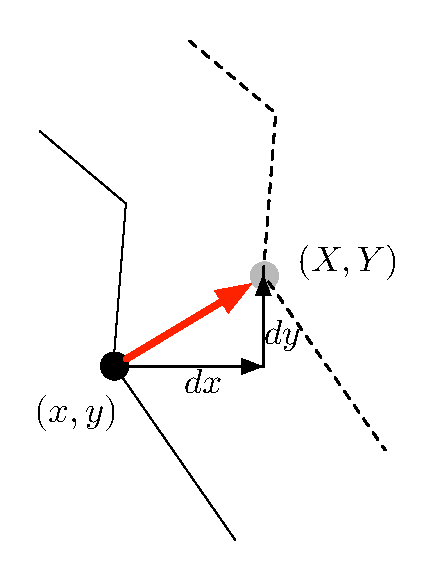
\includegraphics[keepaspectratio,scale=0.7]{img/parallel.eps}\\
    (a)平行移動の原理
   \end{minipage}\\
    \hfill
   \begin{minipage}[b]{0.5\hsize}
    \centering
    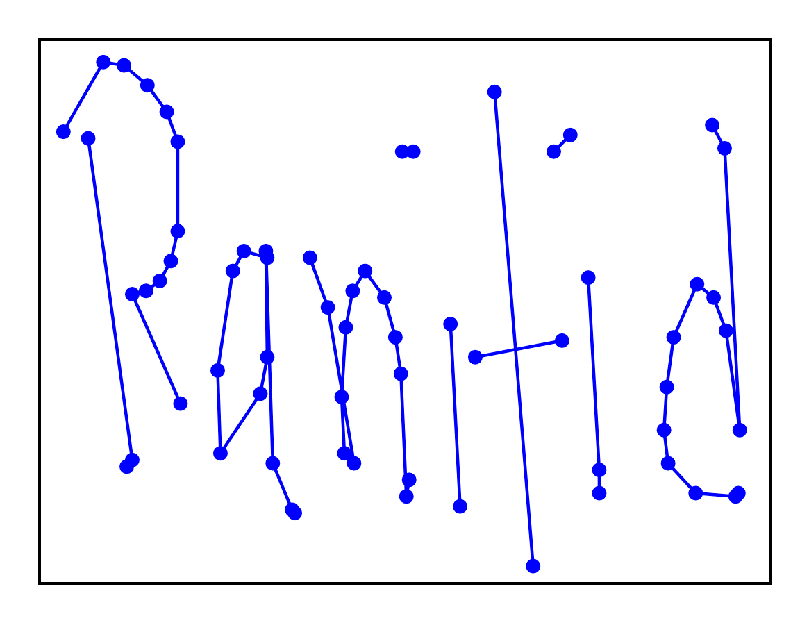
\includegraphics[keepaspectratio,scale=0.5]{img/ranitidCloseBlue.eps}\\
    (b)データ前処理後
   \end{minipage}
   \begin{minipage}[b]{0.5\hsize}
    \centering
    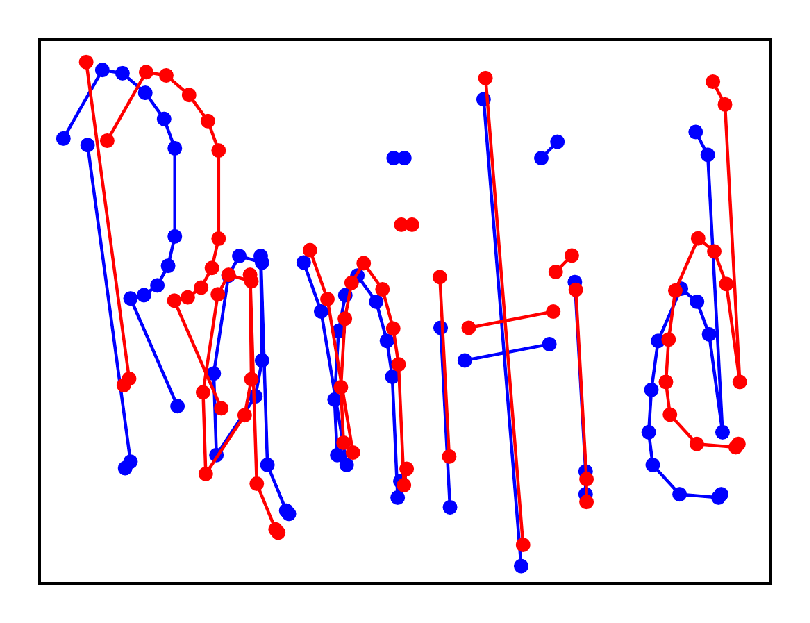
\includegraphics[keepaspectratio,scale=0.5]{img/ranitidParallelRedBlue.eps}\\
    (c)平行移動前(青)と平行移動後(赤)
   \end{minipage}
  \end{tabular}
 \caption{ストロークの平行移動}
 \label{parallel}
\end{figure}



\subsection{Ratio手法}
\label{ratio}
ここでは,オンライン文字におけるデータ拡張の新手法として,文字の縦横比を変更するRatio手法を提案する.先行研究\cite{takahashi}のSRP手法において回転の大きさ,平行移動の大きさは筆者が文字の形を崩さないと判断できる範囲で設定している.そのためデータを100倍に拡張した場合,同じようなデータが増えてしまい学習精度が低くなる原因になる.Ratio手法では文字の縦横比変更を行うので文字のストロークが重なることがなく,文字の形が大きく崩れてしまうことがない.そのため文字の形を崩さない最大のパラメーターでSRP手法を適用した後でも,Ratio手法を用いてさらに拡張できる.またRatio手法は事前に変更比率を定める手法であり,Ratio手法を用いて拡張されたデータはそれぞれが必ず一定の割合で変化しており,少ない倍率でもRatio手法を組み合わせることによってデータが多様化する.SRP手法とRatio手法を組み合わせることによりSRP手法のみで拡張をする場合に比べ,よりデータの多様化を実現することができる.

\textbf{図~\ref{yratio}(a)}に文字の縦横比変更の原理を示す.文字の縦横比変更は$x$座標を基準に行う場合と$y$座標を基準に行う場合がある.
ここでは$y$座標を基準に行う場合を具体的に説明する.1つの単語におけるすべての点のy座標の平均値を取り,すべての点のy座標に対し平均値との大小関係の比較をする.比較結果に応じて,点の移動を行う.文字の拡張比率を$r$,1つの単語上におけるすべての点の$y$座標平均を$\bar{y}$とし,同単語上の任意の点の座標を$(x, y)$としたとき,その点の$y$座標が$\bar{y}$より大きい場合,$y$座標に$y$座標の値の$r$倍を加算し,$\bar{y}$との距離が大きくなる方向に移動させた後の座標$(X, Y)$は 式~\ref{eq:yratio>}で表される.

\begin{equation}
  (X, Y) = (x, y(1+r))
  \label{eq:yratio>}
\end{equation}

一方,$y$座標が$\bar{y}$より小さい場合,$y$座標から$y$座標の値の$r$倍を減算し,$\bar{y}$との距離が大きくなる方向に移動させた後の座標$(X, Y)$は 式~\ref{eq:yratio<}で表される

\begin{equation}
  (X, Y) = (x, y(1-r))
  \label{eq:yratio<}
\end{equation}

この式を単語上のすべての点に用いることで,単語全体の点を単語の$y$座標の平均を基準に移動させ,単語全体を$y$方向に引き伸ばす.
$x$座標を基準に拡張する場合は,これらの式の$x$と$y$を逆にして計算を行う.


\textbf{図~\ref{yratio}(b)}に縦横比率変更前の単語データの例,\textbf{図~\ref{yratio}(c)}に文字の縦横比率を$y$座標を基準に変更後の単語データの例を示す.この処理を,拡張回数ごとに拡張比率$r$と,単語の$x,y$どちらを基準に適応するか変えながら行うことで元のデータとは異なる形の文字・単語を生成する.それを1つの単語データに対して$N$回行い,データ量を$N$倍に拡張する.

$x$座標・$y$座標どちらを基準に比率変更を行うかは$x:y$を$1:2$の割合でランダムに決定している.1つの単語において文字が横方向に並んでいる場合には,全体を$y$座標を基準に縦方向に比率変更を行うのが効果的である.一方単語が1箇所に固まっている場合や斜め方向に書かれている場合には,全体を$x$座標を基準に横方向に比率変更を行うのも効果的であると考えられる.本研究において収集したデータは英語とバングラ語を含んでおり,さらに一般的な文字より雑な文字を扱うため文字の配置が横方向のものだけでなく,斜めや1箇所に集中したものを含んでいる.このため$x:y$を$1:2$の割合とすることでより効果的にデータを多様化させている.

\begin{figure}[tb]
 \centering
  \begin{tabular}{c}
   \begin{minipage}[b]{0.7\hsize}
    \centering
    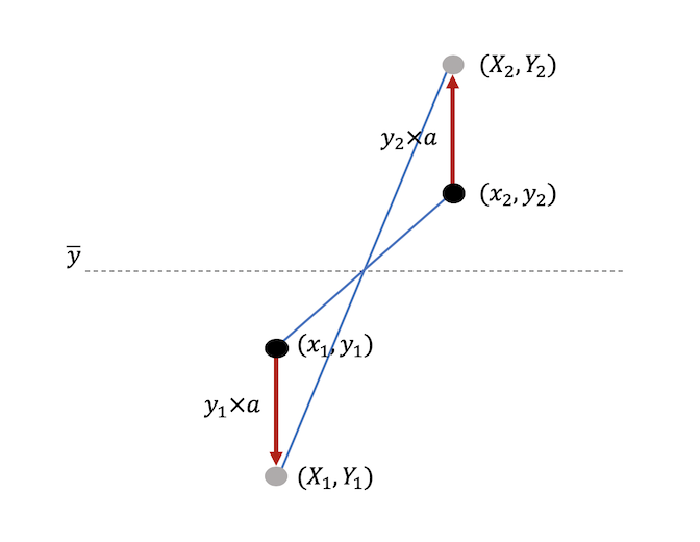
\includegraphics[keepaspectratio,scale=0.7]{img/yratio.eps}\\
    (a)縦横比率変更の原理
   \end{minipage}\\
    \hfill
   \begin{minipage}[b]{0.5\hsize}
    \centering
    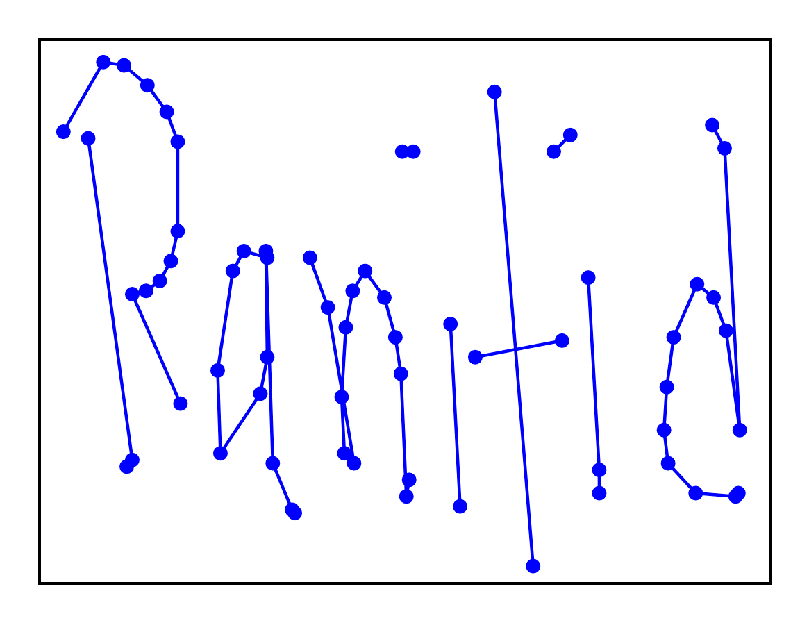
\includegraphics[keepaspectratio,scale=0.5]{img/ranitidCloseBlue.eps}\\
    (b)データ前処理後
   \end{minipage}
   \begin{minipage}[b]{0.5\hsize}
    \centering
    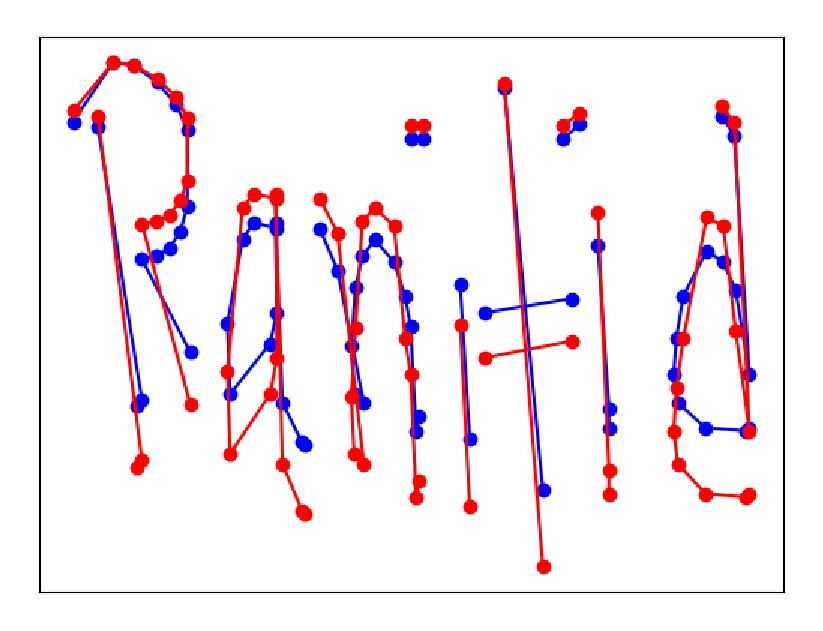
\includegraphics[keepaspectratio,scale=0.5]{img/ranitidRatioRedBlue.eps}\\
    (c)縦横比率変更前(青)と変更後(赤)
   \end{minipage}
  \end{tabular}
 \caption{文字の縦横比率変更}
 \label{yratio}
\end{figure}


\section{機械学習ブロック}
\label{sec:m_learning}
本論文ではBidirectionalLSTMを用いて学習を行う.\textbf{図~\ref{blstm}}にBidirectionalLSTMの概要を示す.BidirectionalLSTMは従来のLSTMに未来の入力から計算を行う逆方向のモデルを加え,出力を同一の出力層に統合するものである.学習プロセスでは,データ拡張が施された直線データを入力として用いる.本論文においてBidirectionalLSTMは,現在入力されている直線データより前に書かれた直線データだけでなく,後に書かれる直線データも用いて学習を行う.推定プロセスでは,学習が行われたモデルに前処理後のデータを入力し,用語の推定を行う.

学習モデルは先行研究を参考に作成し,実装にはpythonのニューラルネットワークライブラリであるKeras\cite{keras}を用いている.活性化関数にはSoftmax関数\cite{softmax}を用いて出力を確率として解釈し,最も確率の高い項目を予測値として決定している.損失関数にはcategorical\_crossentropy\cite{categoricalcrossentropy},最適化関数にはAdam\cite{kingma14:adam}を用いており,学習の評価は正解率で計算を行なっている.

\begin{figure}[tb]
 \begin{center}
  \resizebox{\columnwidth}{!}{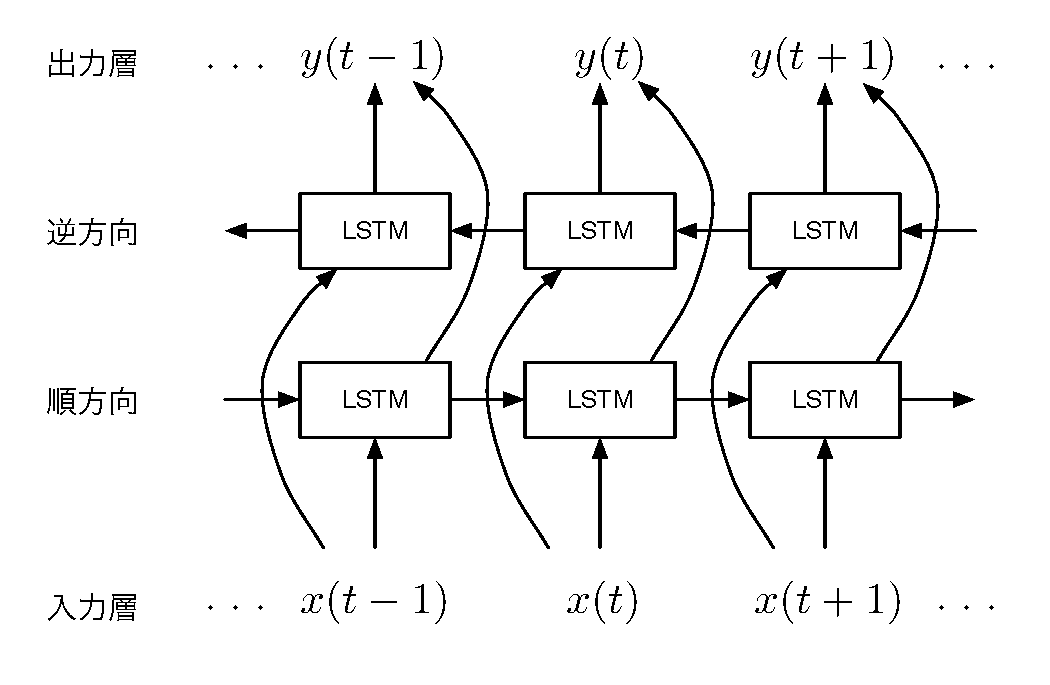
\includegraphics{img/blstm.eps}}
  \caption{BidirectionalLSTMの概要}
  \label{blstm}
\end{center}
\end{figure}

% 以下はRefTeX用
%%% Local Variables:
%%% mode: yatex
%%% TeX-master: "thesis"
%%% End:
